% !TEX root = ./main.tex

\documentclass{article}
\usepackage[utf8]{inputenc}
\usepackage[ngerman]{babel}
\usepackage{pdfpages}
\usepackage{graphicx}
\usepackage{amsmath}
\graphicspath{ {./img/} }

\usepackage{lipsum}
\usepackage{float}
\usepackage{listings}

\usepackage{xcolor}

\definecolor{codegreen}{rgb}{0,0.6,0}
\definecolor{codegray}{rgb}{0.5,0.5,0.5}
\definecolor{codepurple}{rgb}{0.58,0,0.82}
\definecolor{backcolour}{rgb}{0.95,0.95,0.92}

\lstdefinestyle{mystyle}{
    backgroundcolor=\color{backcolour},   
    commentstyle=\color{codegreen},
    keywordstyle=\color{magenta},
    numberstyle=\tiny\color{codegray},
    stringstyle=\color{codepurple},
    basicstyle=\ttfamily\footnotesize,
    breakatwhitespace=false,         
    breaklines=true,                 
    captionpos=b,                    
    keepspaces=true,                 
    numbers=left,                    
    numbersep=5pt,                  
    showspaces=false,                
    showstringspaces=false,
    showtabs=false,                  
    tabsize=2
}

\lstset{style=mystyle}
\lstset{literate=%
{Ö}{{\"O}}1
{Ä}{{\"A}}1
{Ü}{{\"U}}1
{ß}{{\ss}}2
{ü}{{\"u}}1
{ä}{{\"a}}1
{ö}{{\"o}}1
}

\newcommand{\nr}{1}


\title{Aktorik Sensorik \\ Labor 1}
\author{Anton Kress (S872899), Jan Abel (S876662)}
\date{October 2020}

\begin{document}

\maketitle

\newpage
\tableofcontents 
\section{Labor 2}

\subsection{Einleitung und Ziel}

Im 2. Labor im Modul Aktorik und Sensorik soll die Ankerinduktiviät $L$
und die Reibungskonstante $c_r$ eines Gleichstrommotors bestimmt werden.

\subsection{Grundlagen und Theorie}
\subsection{Aufgabenstellung und Versuch}

\subsubsection{Bestimmung der Ankerinduktivität}

Um die Ankeridnuktivität zu bestimmen, muss der Motor gebremst sein,
damit die induzierte Gegenspannung $U_{ind} = 0$ ist. Dann ergibt sich
folgendes Schaltbild.


\begin{figure}[H]
    \centering
    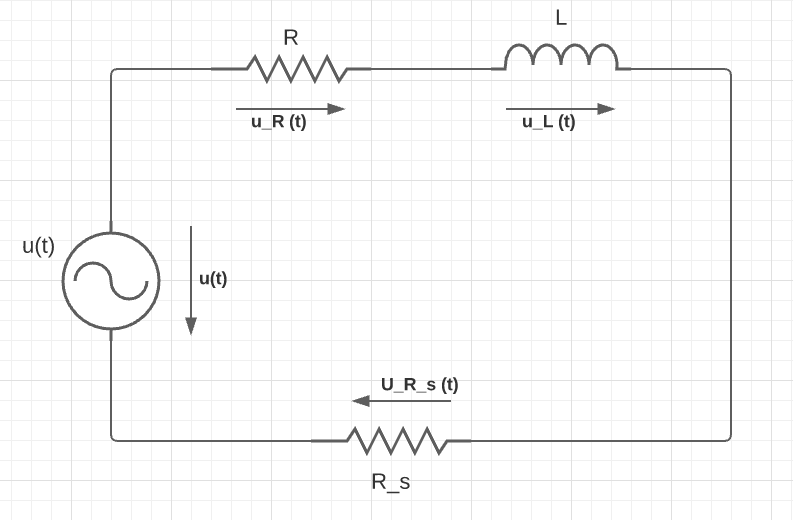
\includegraphics[width=1\textwidth]{schaltplan.png}
    \caption{Mess-Schaltung Ankerinduktivität}
    \label{fig:PlotAufgabe1}
   \end{figure}

Diese Schaltung kann durch folgende Maschengleichung beschrieben werden.

\begin{equation} \label{eq211}
    \begin{split}
        u(t)&=u_R(t) + u_L(t)\\
        u(t)&=R \cdot i(t) + L \frac{d i(t)}{dt}\\
        u(t)&= (R+R_s) \cdot i(t) + L \frac{d i(t)}{dt}
    \end{split}
\end{equation}

Die Idee zur Bestimmung der Induktivität ist nun folgende. Die Schaltung
wird mit einer sinusförmigen Wechselspannung betrieben. Über die
Phasenverschiebung der Eingangsspannung und des Stromes kann die Induktivität
bestimmt werden.

\begin{equation} \label{eq212}
    \begin{split}
        \underline{U} = A \cdot e^{\jmath 0}\\
        \underline{I} = B \cdot e^{\jmath \varphi}
    \end{split}
\end{equation}

Der Strom $i(t)$ wird indirekt über den Messwiderstand $R_s= 1\Omega$
bestimmt, da folgendes gilt.

\begin{equation} \label{eq213}
    \begin{split}
        i(t)=\frac{u_{Rs}(t)}{R_s} = u_{Rs}(t)
    \end{split}
\end{equation}

Der Phasenwinkel kann über die Impedanz $\underline{Z}$ berechnet werden.

\begin{equation} \label{eq214}
    \begin{split}
        \underline{Z} &= (R + R_s) + \jmath \omega L\\
        \varphi\{\underline{Z} \} &= \arctan \left( \frac{\omega L}{ R + R_s} \right)
    \end{split}
\end{equation}

Da nicht der Phasenwinkel $\varphi$ sondern die Phasenverschiebung $\Delta t$ gemessen
wird, muss dieser noch umgerechnet werden.

\begin{equation} \label{eq215}
    \begin{split}
        \varphi &= \frac{\Delta t}{T} \cdot 2 \pi \\
        \varphi &=  \omega \Delta t = 2 \pi f \Delta t
    \end{split}
\end{equation}

Nun lässt sich die Induktivität $L$ folgendermaßen berechnen.

\begin{equation} \label{eq216}
    \begin{split}
        L = \frac{(R+R_s) }{2 \pi f} \cdot \tan(2 \pi f \Delta t)
    \end{split}
\end{equation}

Da in der Messung die Phasenverschiebung $\Delta t$ in Abhängigkeit
von der Frequenz $f$ gemessen worden ist, ergibt sich die Funktion $f_1(f)$.

\begin{equation} \label{eq217}
    \begin{split}
       \Delta t = f_1(f) = \frac{1}{2 \pi f} \arctan \left( \frac{2 \pi L}{R + R_s} f \right)
    \end{split}
\end{equation}

Um diese Funktion zu Linearisieren muss diese noch umgestellt werden.

\begin{equation} \label{eq218}
    \begin{split}
       \tan(2 \pi f \Delta t) = f_2(f) = \frac{2 \pi L}{R + R_s} f
    \end{split}
\end{equation}

Nun kann mittels der linearen Regression aus den beiden Vektoren die Steigung
$m$ bestimmt werden, aus der sich die Induktivität $L$ berechnen lässt.

\begin{equation} \label{eq219}
    \begin{split}
       m &=  \frac{2 \pi L}{R + R_s}\\
       L &= \frac{m \cdot (R+R_s)}{2 \pi} \simeq 175.462 \mathrm{\mu H}
    \end{split}
\end{equation}


\begin{figure}[H]
 \centering
    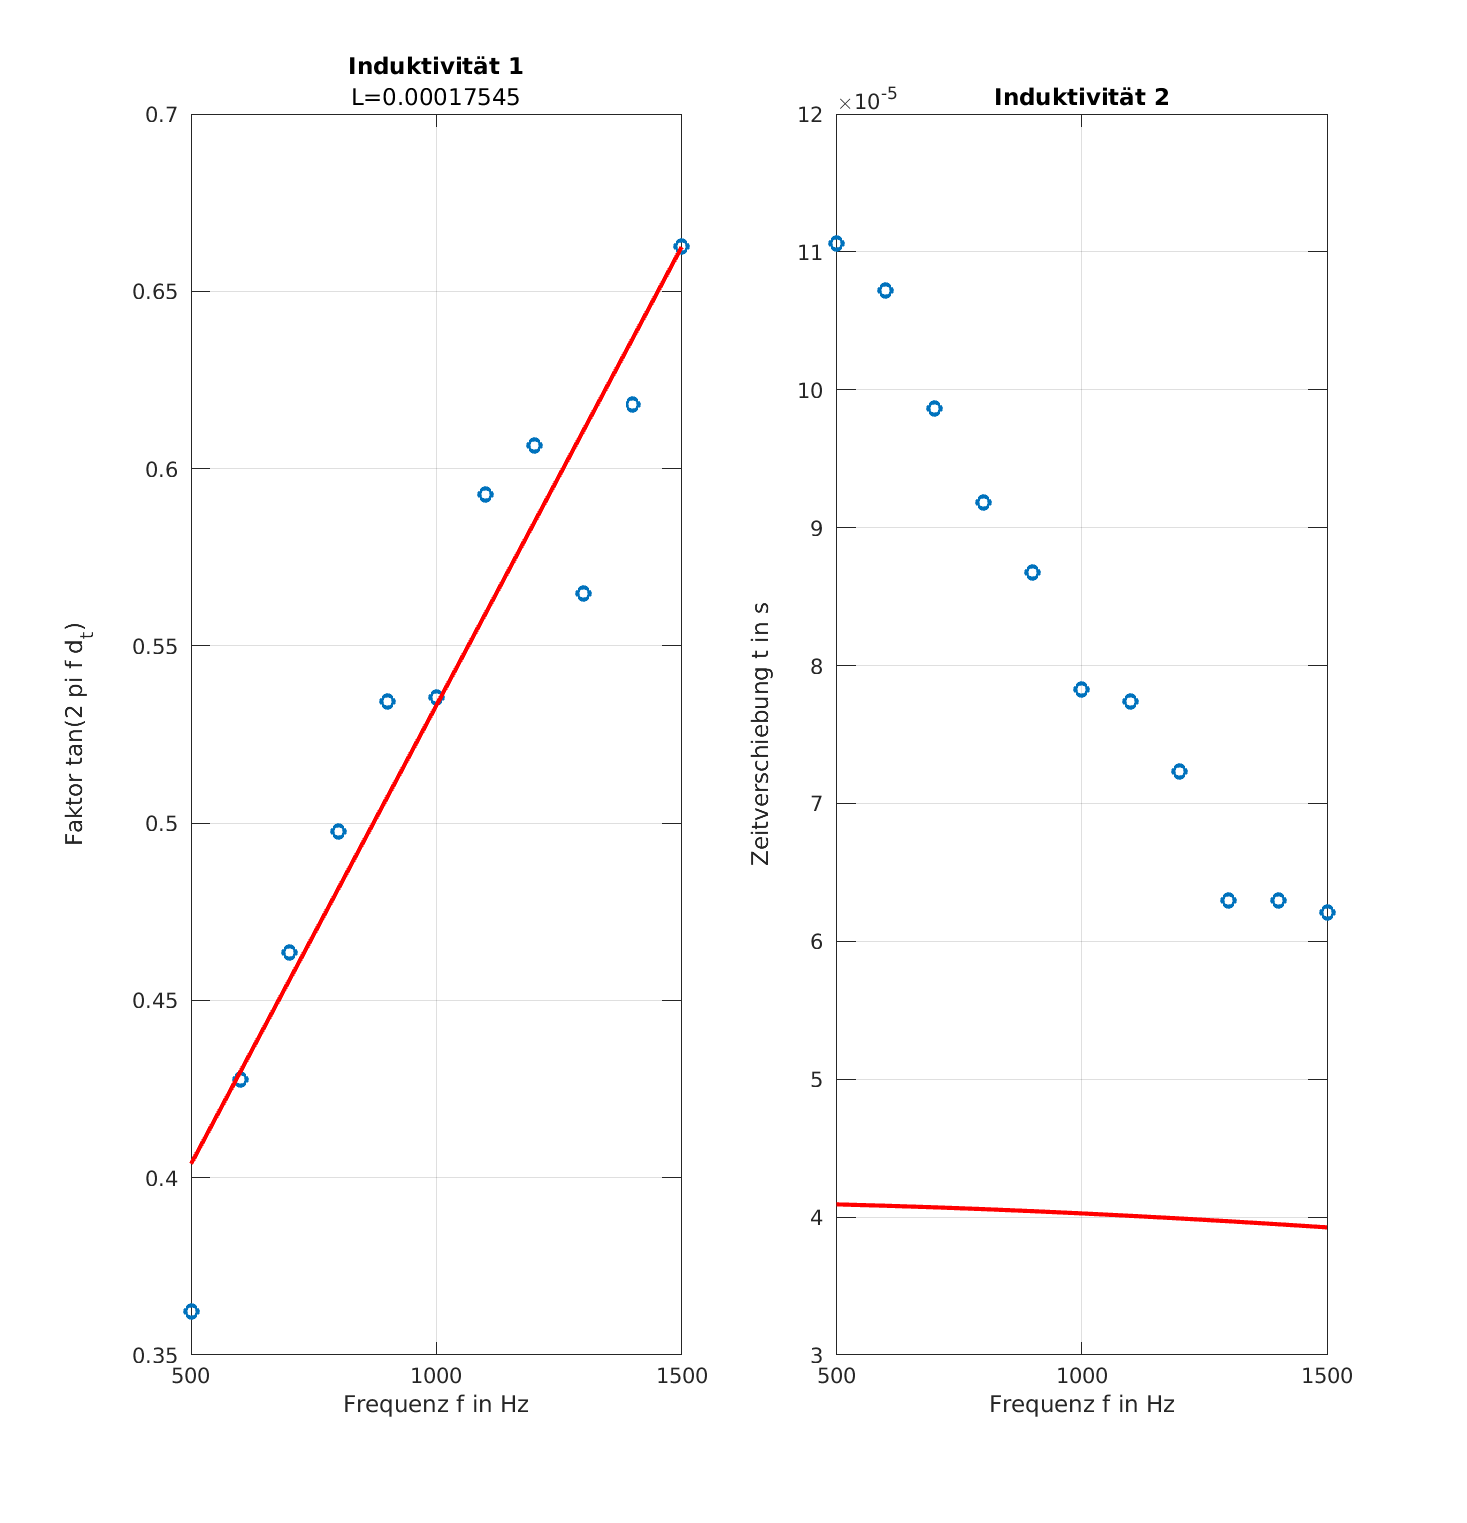
\includegraphics[width=1\textwidth]{as_labor02_1.png}
 \caption{Plot der Aufgabe 1}
 \label{fig:PlotAufgabe1}
\end{figure}
\subsubsection{Bestimmung der Reibungskonstanten}

Die Reibungskonstante kann über folgende DGL berechnet werden.
Die Summe der Drehmomente ergibt sich aus dem Drehmoment $M_m$
abzüglich des Reibungsdrehmoments $M_R$ und des Lastdrehmoments.
Diese sind gleich der zeitlichen Änderung der Winkelgeschwindikeit 
$\frac{d \omega}{dt}$ multipliziert mit dem Trägheitsmoment $J$.

\begin{equation} \label{eq221}
    \begin{split}
        J \frac{d \omega}{d t} &= \sum M = M_m - M_R - M_L \\
        J \frac{d \omega}{d t} &= \sum M = k_m \cdot i(t) - c_r \omega (t) - M_L 
    \end{split}
\end{equation}

Um die Reibungskonstante $c_r$ nun zu bestimmen, ist es günstig das
System im Leerlauf zu betrachten, da $M_L=0$ und nach Abklingen des
Einschaltvorgangs $\frac{d\omega}{dt} =0$. Aus der DGL ergibt sich
folgende einfache Gleichung.

\begin{equation} \label{eq222}
    \begin{split}
        0 & = k_m \cdot i(t) - c_r \omega (t)
    \end{split}
\end{equation}

Daraus ergibt sich folgende Funktion.

\begin{equation} \label{eq222}
    \begin{split}
        \omega = f_3(i) = \frac{k_m}{c_r} i
    \end{split}
\end{equation}

Nun kann mittels der linearen Regression aus den beiden Vektoren die Steigung
$m$ bestimmt werden, aus der sich die Reibungskonstante $c_r$ berechnen lässt.

\begin{equation} \label{eq218}
    \begin{split}
       m &=  \frac{k_m}{c_r}\\
       c_r &= \frac{k_m}{m} \simeq 3,24 \cdot 10^{-9} \mathrm{\frac{Nm s}{rad}}
    \end{split}
\end{equation}

\begin{figure}[H]
 \centering
    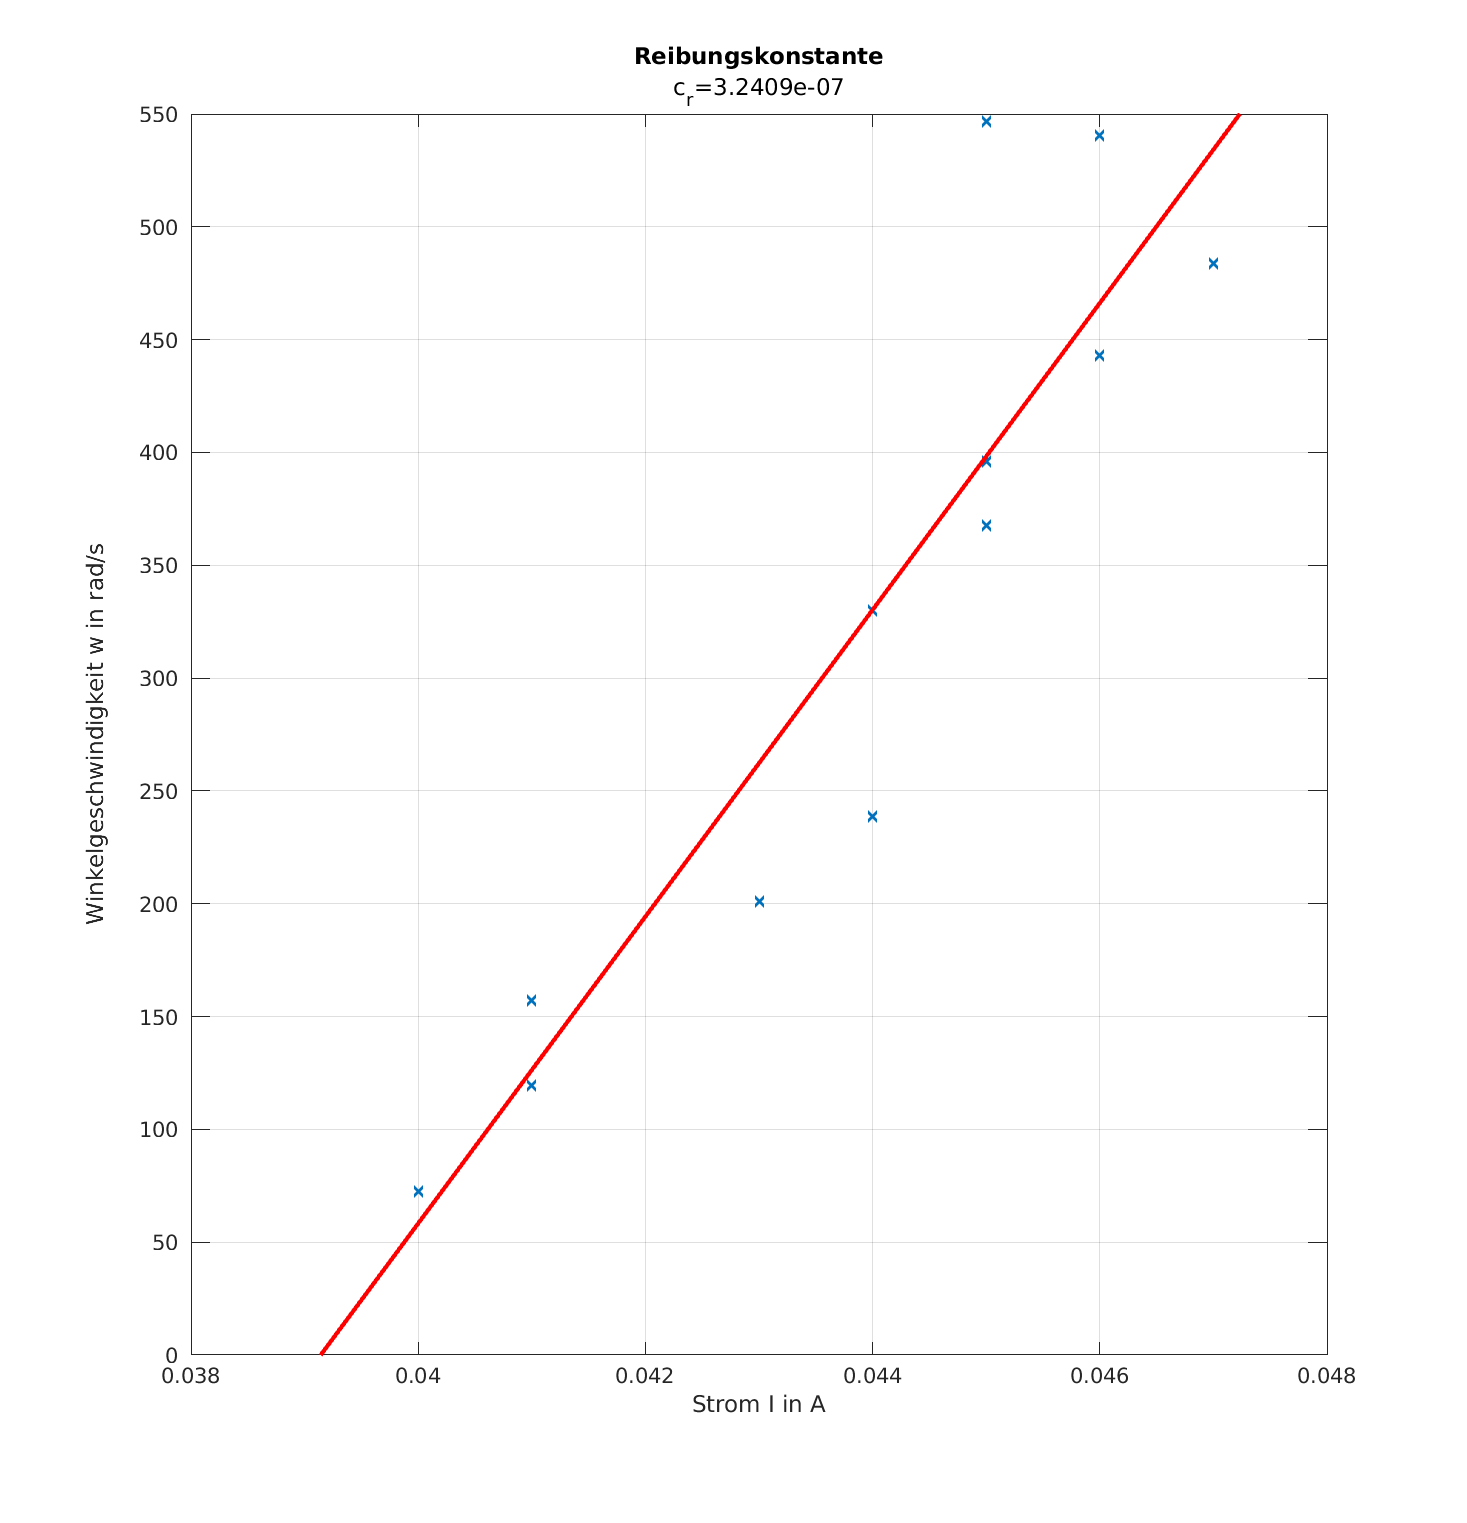
\includegraphics[width=1\textwidth]{as_labor02_2.png}
 \caption{Plot der Aufgabe 1}
 \label{fig:PlotAufgabe1}
\end{figure}
%\subsection{Zusammenfassung}

Mittels der Messwerte sind wir auf folgende Werte für die Ankerinduktivität $L$
und die Reibungskonstante $c_r$ gekommen.

\begin{equation} \label{eq241}
    \begin{split}
       L &=  175.462 \mathrm{\mu H}\\
       c_r &= 3,24 \cdot 10^{-9} \mathrm{\frac{Nm s}{rad}}
    \end{split}
\end{equation}

Die Berechnung der Reibungskonstante stellte uns vor keine Herausforderung
und ist sowohl Einheitenmäßig als auch Dimensionsmäßig nachvollziehbar.\\

Die Bestimmung der Ankerinduktivität stellte uns allerdings vor die
Herausforderung das System zu liniearisieren (Abbildung 2: Induktivität 1).
Nach der Liniearisierung der Funktion und anschließender Regression haben wir
den errechneten Wert der Induktivität wieder in die Ursprungsfunktion eingesetzt
(Abbildung 2: Induktivität 2). Hier ist zu erkennen, dass die ermittelte Gerade
sich nur bedingt in der Nähe der Messpunkte befindet. Wir vermuten, dass entweder
eine Ungenauigkeit in unseren Modell vorhanden ist oder es ist einen vielleicht
sogar frequenzabhängigen Offset in den Messdaten gibt. Um dieses Verhalten genauer
zu untersuchen, haben wir die Funktion und die Messdaten \href{https://www.desmos.com/calculator/2je7stqm76}{interaktiv in Desmos}
erstellt.\\

Wir konnten diese Diskrepanz leider nicht abschließend klären, sind aber zum Entschluss
gekommen das unser Ergebnis von $175.462 \mathrm{\mu H}$ ausreichend genau und auch realistisch ist.
\subsection{Anhang}

\subsubsection{Aufgabenbeschreibung}
\begin{figure}[H]
    \centering
    \includegraphics[page=5, width=0.8\textwidth]{../Aufgabenstellung.pdf}
    %\caption{caption}
    \label{fig:Aufgabenstellung Labor 2.1}
\end{figure}

\begin{figure}[H]
    \centering
    \includegraphics[page=6, width=0.8\textwidth]{../Aufgabenstellung.pdf}
    \label{fig:Aufgabenstellung Labor 2.2}
\end{figure}

\subsubsection{Matlab Code}
\lstinputlisting[language=Matlab]{matlab/as_labor02_1.m}
\lstinputlisting[language=Matlab]{matlab/as_labor02_2.m}

%\subsubsection{Messwerte}

\end{document}
